\section{Results} 
\subsection{Optimal \(\epsilon\) selection}

In order to analyze the data generated by the planner \(d_J\) is plotted against a varying \(\epsilon\).
The results have a skewed variation towards an infinite long path length as infinite trials will never yield a zero path length.
Thus a median was found in order to compare the performance.
In figure \ref{fig:bidir_correlated} can the distance of the trials for bidirectional RRT be seen with the median highlighted.
In figure \ref{fig:balanced_correlated} can the results be seen for the balanced bidirectional RRT.

The Spearman's Rank Correlation, with the null-hypothesis that \(d_J\) is uncorrelated with \(\epsilon\) gave a p-value of \(1\cdot 10^{-19}\) for the bidirectional and a p-value of \(6\cdot 10^{-21}\) for the balanced bidirectional RRT.
This means in both cases are the \(d_J\) and \(\epsilon\) correlated.

To give each algorithm the best chance to provide the optimal path, the optimal \(\epsilon\) was found for both algorithms.
The optimal \(\epsilon\) was found by taking the lowest median.
For Bidirectional, the optimal \(\epsilon\) was found to be 2.25 and for Balanced Bidirectional it was found to be 2.15.

\begin{figure}[h]
 \centering
 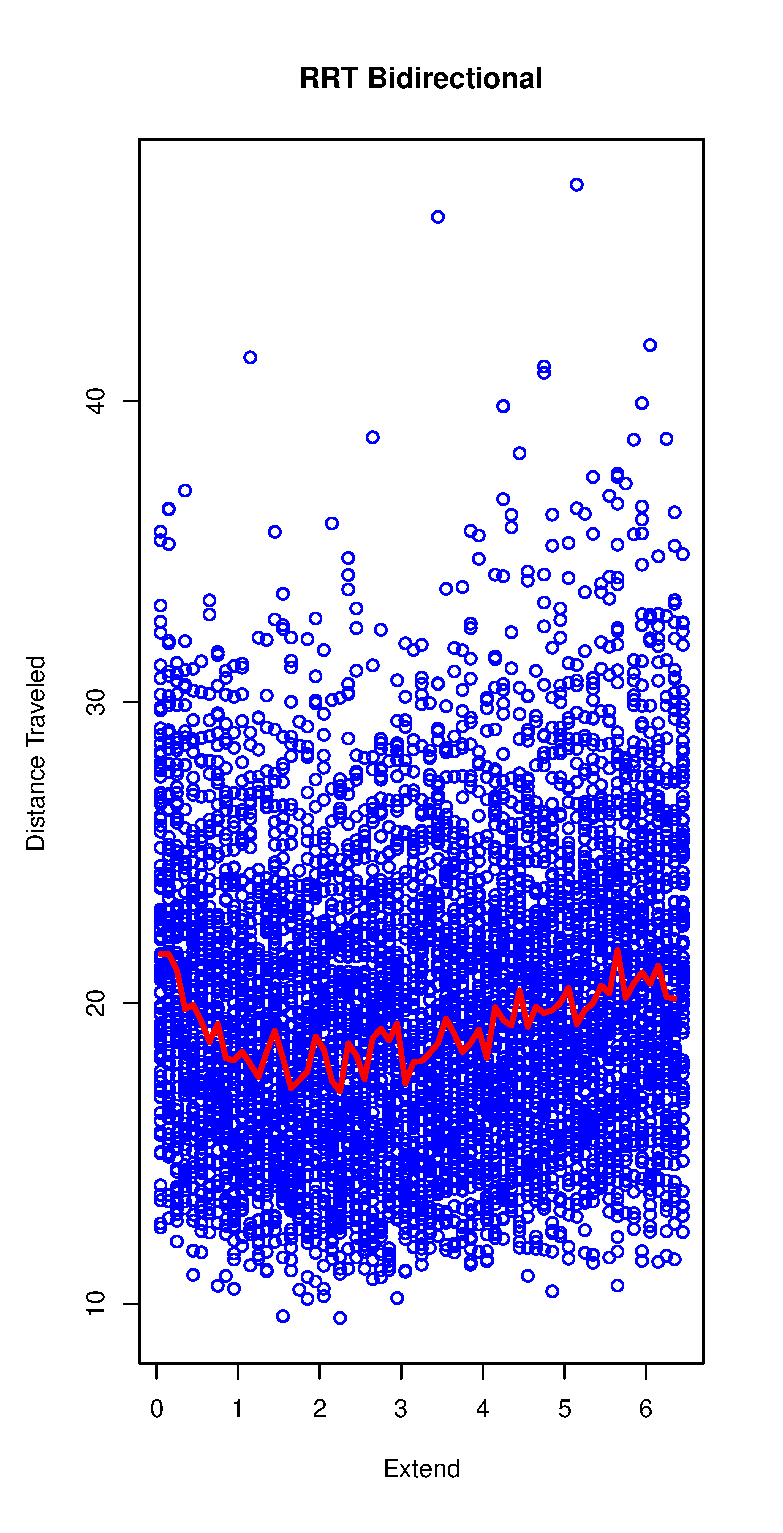
\includegraphics[width=\figsize]{graphics/bidirectional_correlation}
 \caption{\(d_J\) of the bidirectional RRT planner (blue) with median highlighted (red).}
 \label{fig:bidir_correlated}
\end{figure}

\begin{figure}[h]
 \centering
 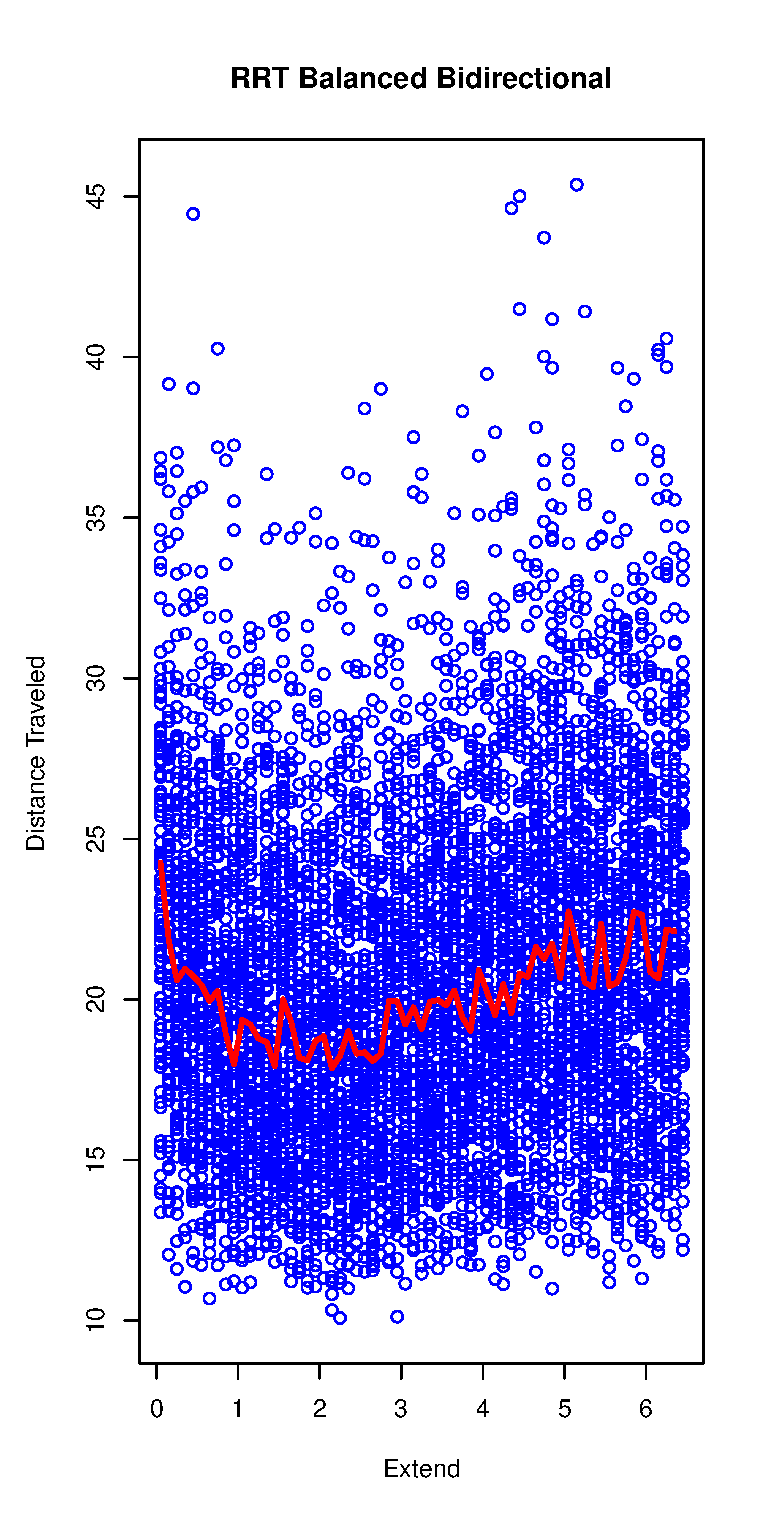
\includegraphics[width=\figsize]{graphics/balanced_correlation}
 \caption{\(d_J\) of the balanced bidirectional RRT planner (blue) with median highlighted (red).}
 \label{fig:balanced_correlated}
\end{figure}

In figure \ref{fig:medians} can the median distances be seen. 
The median distance is observed to be higher on the balanced bidirectional. 
Whether the difference is significant requires further investigation.

\begin{figure}[h]
 \centering
 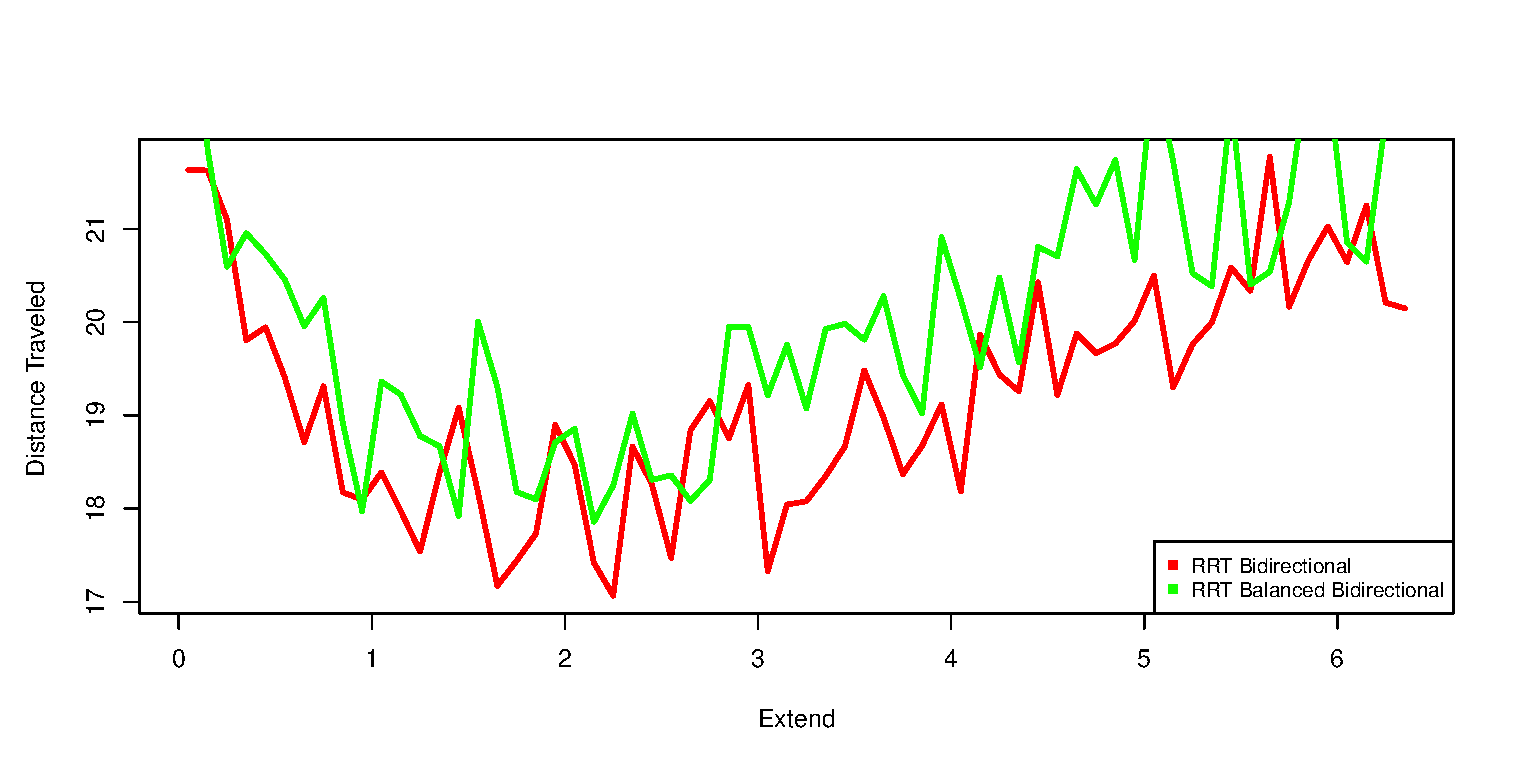
\includegraphics[width=\figsize]{graphics/compare_distance}
 \caption{Medians of \(d_J\) for the RRT planners.}
 \label{fig:medians}
\end{figure}

\subsection{Algorithm comparison}

By plotting the histogram of the path length with the optimal \(\epsilon\), as seen in figure \ref{fig:bidir_histogram} and \ref{fig:balanced_histogram}, it can be seen that it is not normally distributed. 
From the QQ plot it can be seen that the correlation between a normal distribution is exponential.
The data is transformed into log space.
The QQ plots of the transformed data looks linear, but to be certain is a shapiro wilks test applied to test for normality.
The p-value for the bidirectional was \(1.5\cdot10^{-3}\) and for the balanced bidirectional it was \(4.2\cdot10^{-4}\).
This suggest the data is still not normally distributed.
To test if the variances are equal, an F test is applied.
The p-value is  \(0.087\), the variance is significantly different.

Since the variances are different, the method to test if the mean is different, is the Welch's t-test.
The p-value is:  0.10, the mean are significantly different, the bidirectional RRT is the better planner in a confined space.

\begin{figure}[h]
 \centering
 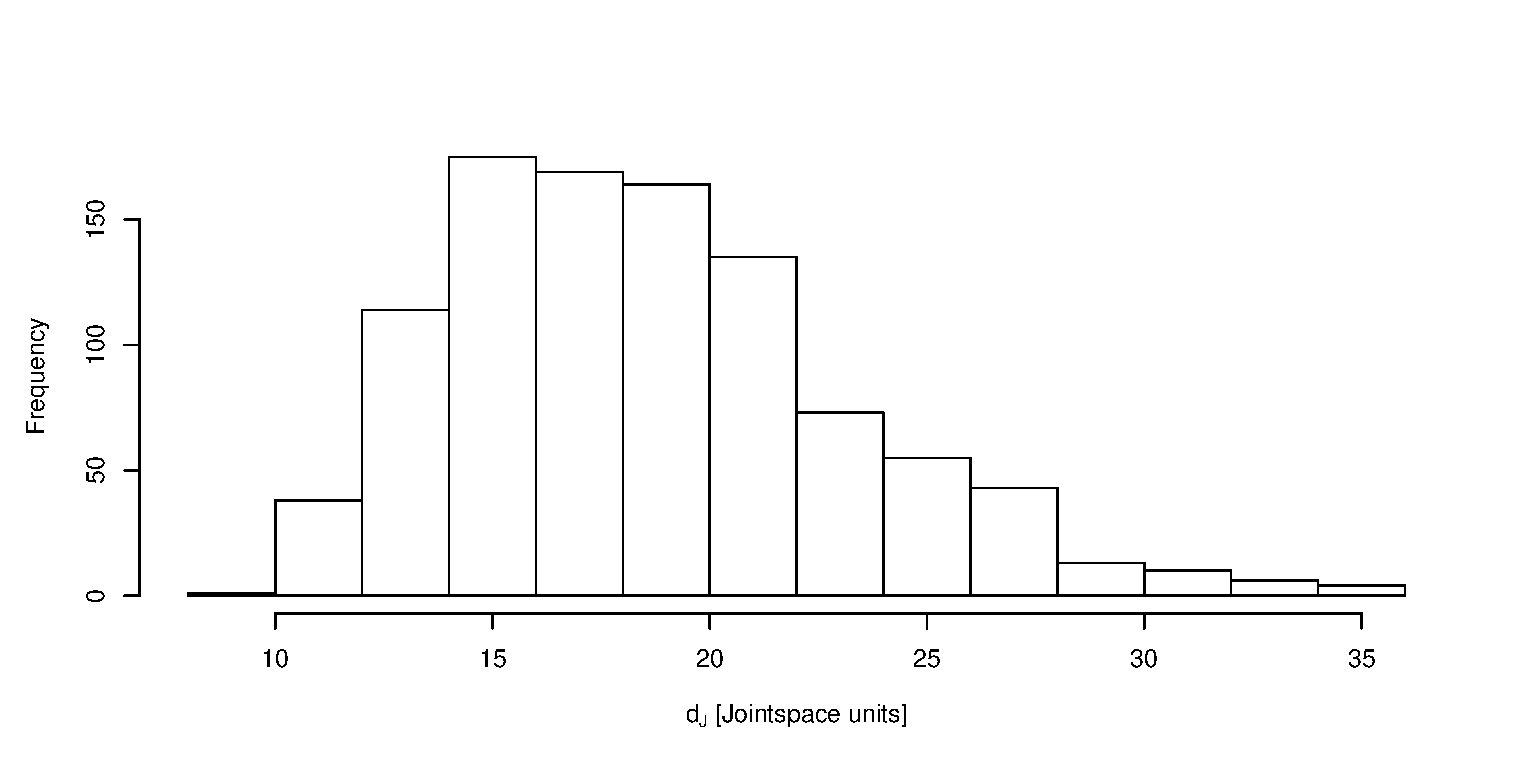
\includegraphics[width=\figsize]{graphics/hist_op_bi}
 \caption{Histogram for \(d_J\) with the optimal \(\epsilon\) for the bidirectional RRT planner.}
 \label{fig:bidir_histogram}
\end{figure}

\begin{figure}[h]
 \centering
 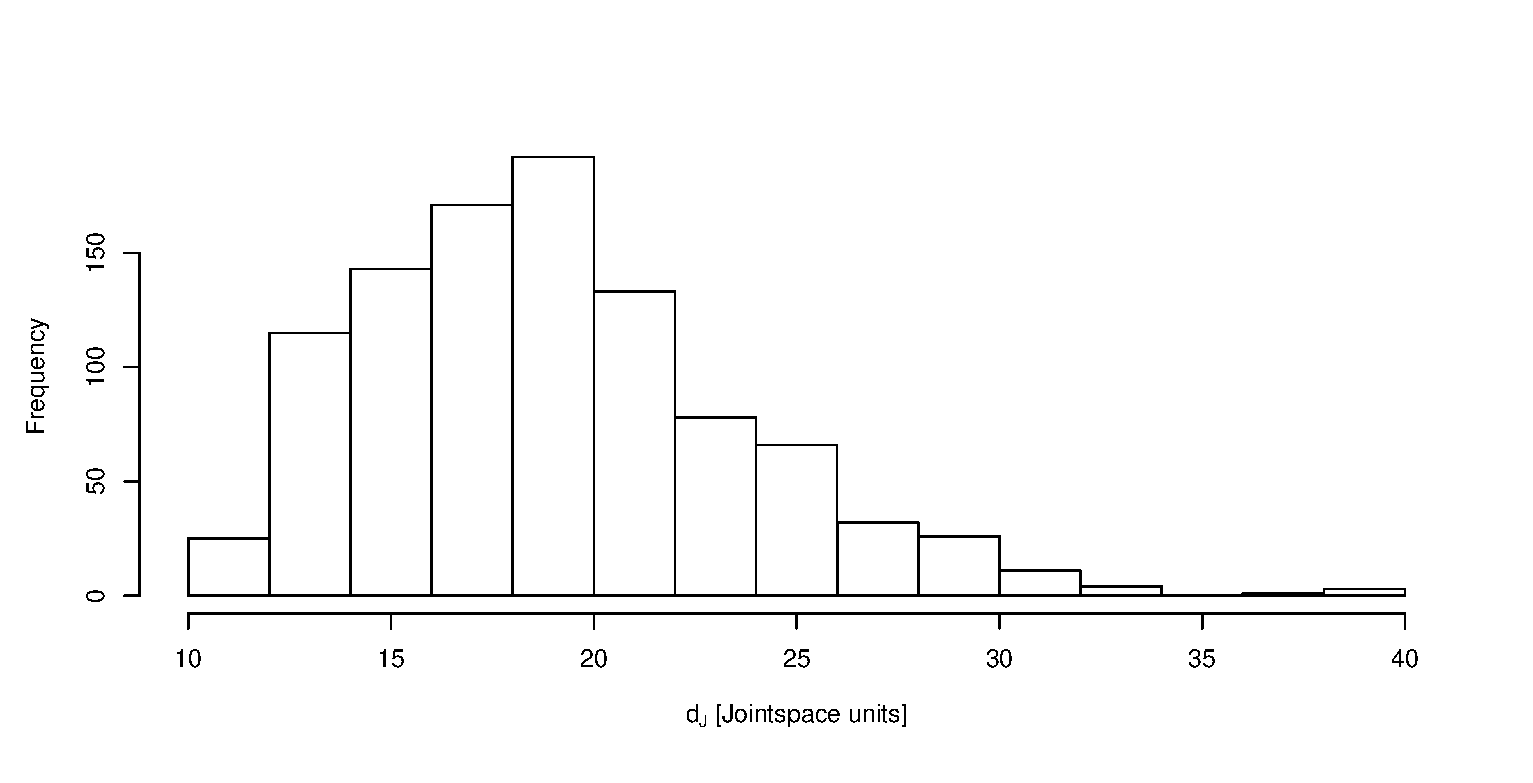
\includegraphics[width=\figsize]{graphics/hist_op_ba}
 \caption{Histogram for \(d_J\) with the optimal \(\epsilon\) for the balanced bidirectional RRT planner.}
 \label{fig:balanced_histogram}
\end{figure}

\begin{figure}[h]
 \centering
 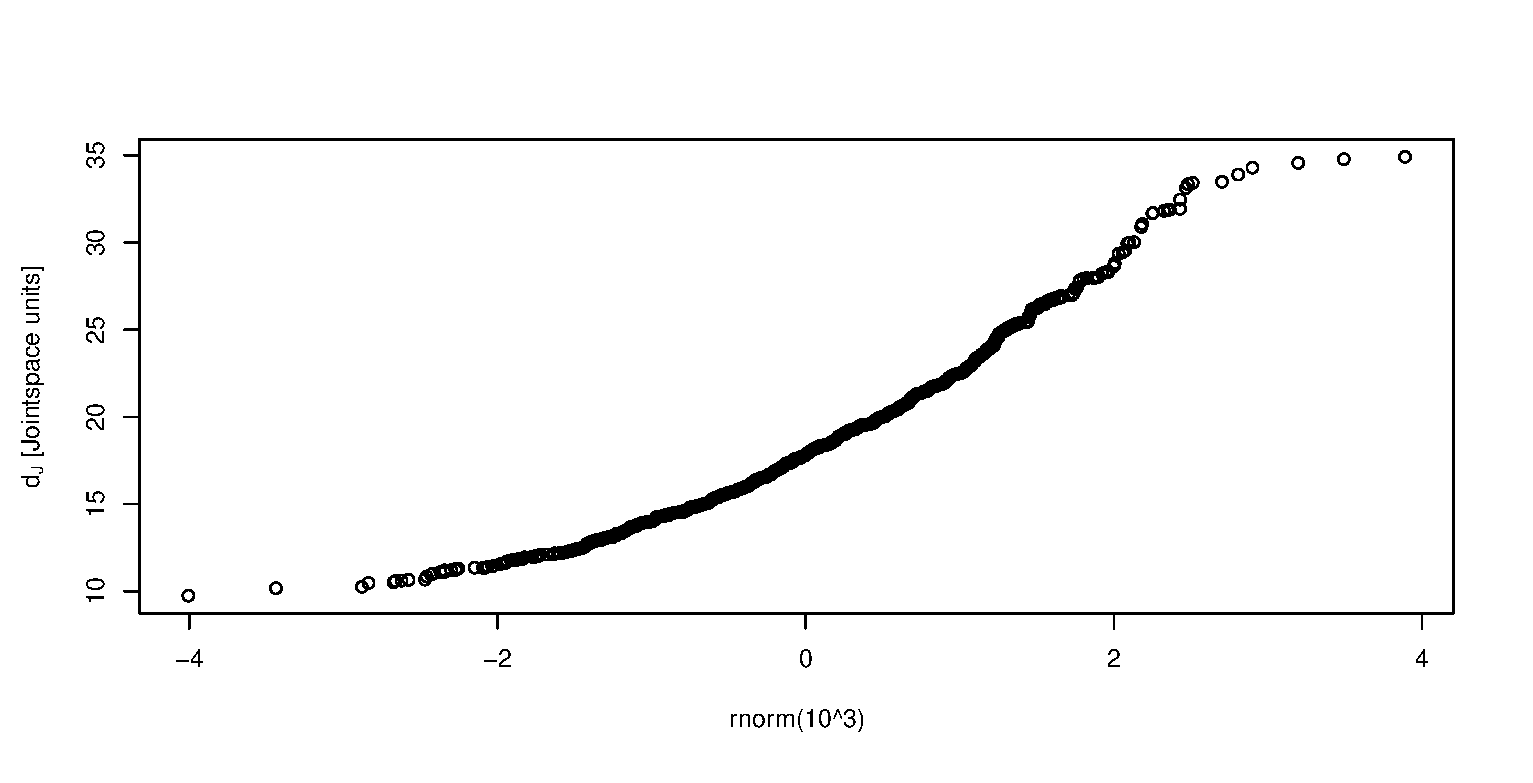
\includegraphics[width=\figsize]{graphics/qq_op_bi}
 \caption{Normal QQ plot for \(d_J\) with the optimal \(\epsilon\) for the bidirectional RRT planner. The normal distribution is approximated with 1000 samples.}
 \label{fig:bidir_qq}
\end{figure}

\begin{figure}[h]
 \centering
 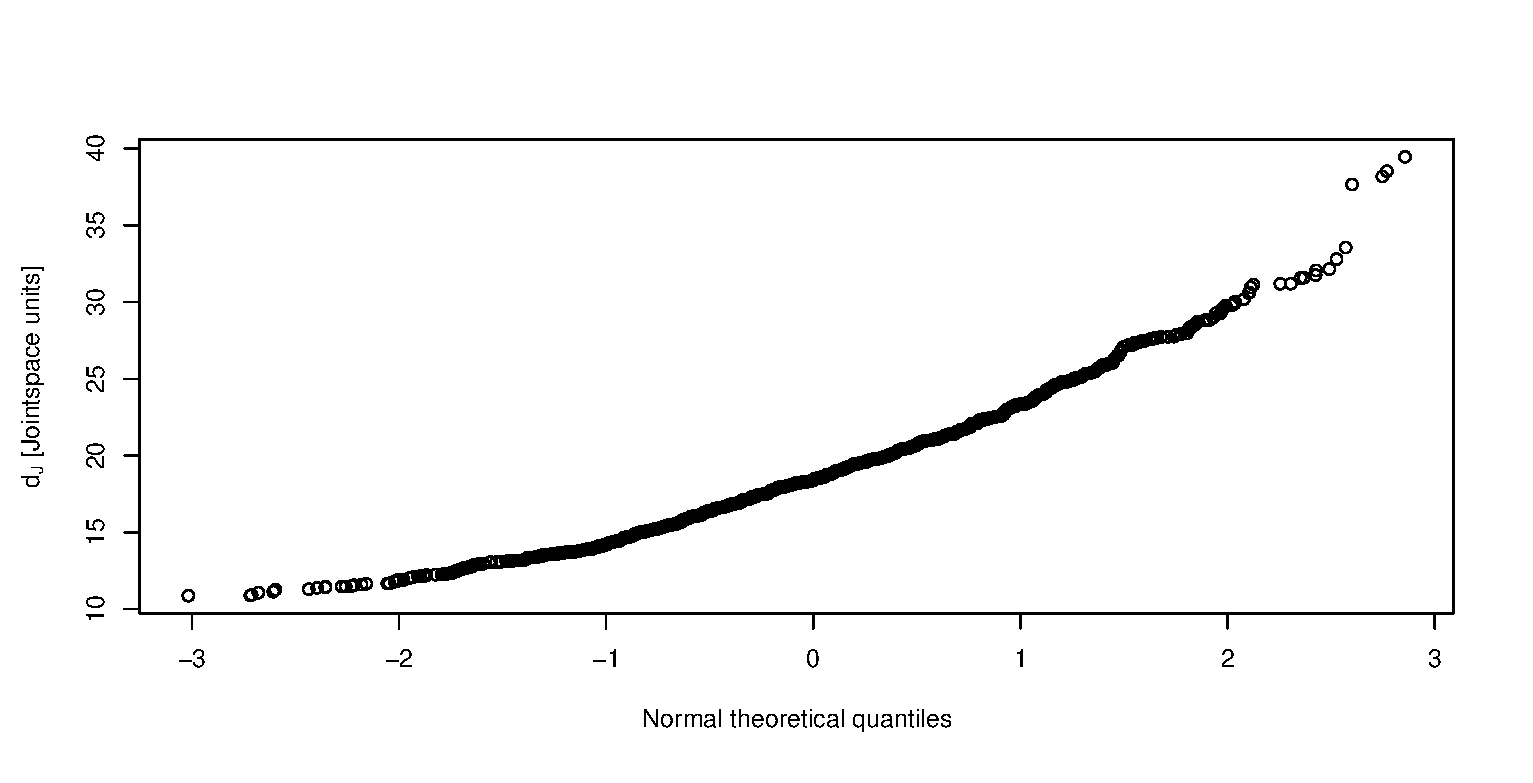
\includegraphics[width=\figsize]{graphics/qq_op_ba}
 \caption{Normal QQ plot for \(d_J\) with the optimal \(\epsilon\) for the balanced bidirectional RRT planner. The normal distribution is approximated with 1000 samples.}
 \label{fig:balanced_qq}
\end{figure}

\begin{figure}[h]
 \centering
 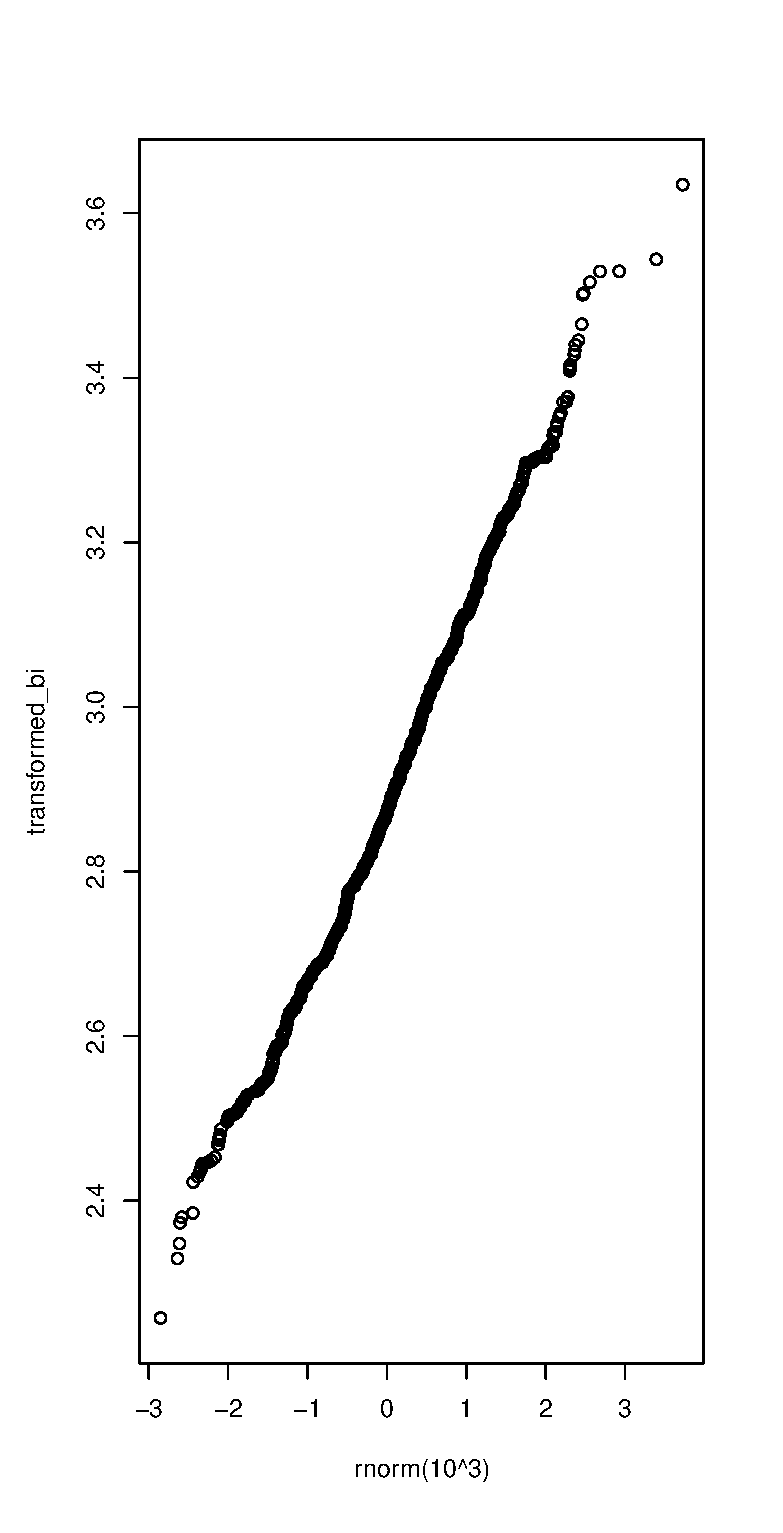
\includegraphics[width=\figsize]{graphics/qq_tran_op_bi}
 \caption{Normal QQ plot for the log transformed \(d_J\) with the optimal \(\epsilon\) for the bidirectional RRT planner. The normal distribution is approximated with 1000 samples.}
 \label{fig:bidir_log_qq}
\end{figure}

\begin{figure}[h]
 \centering
 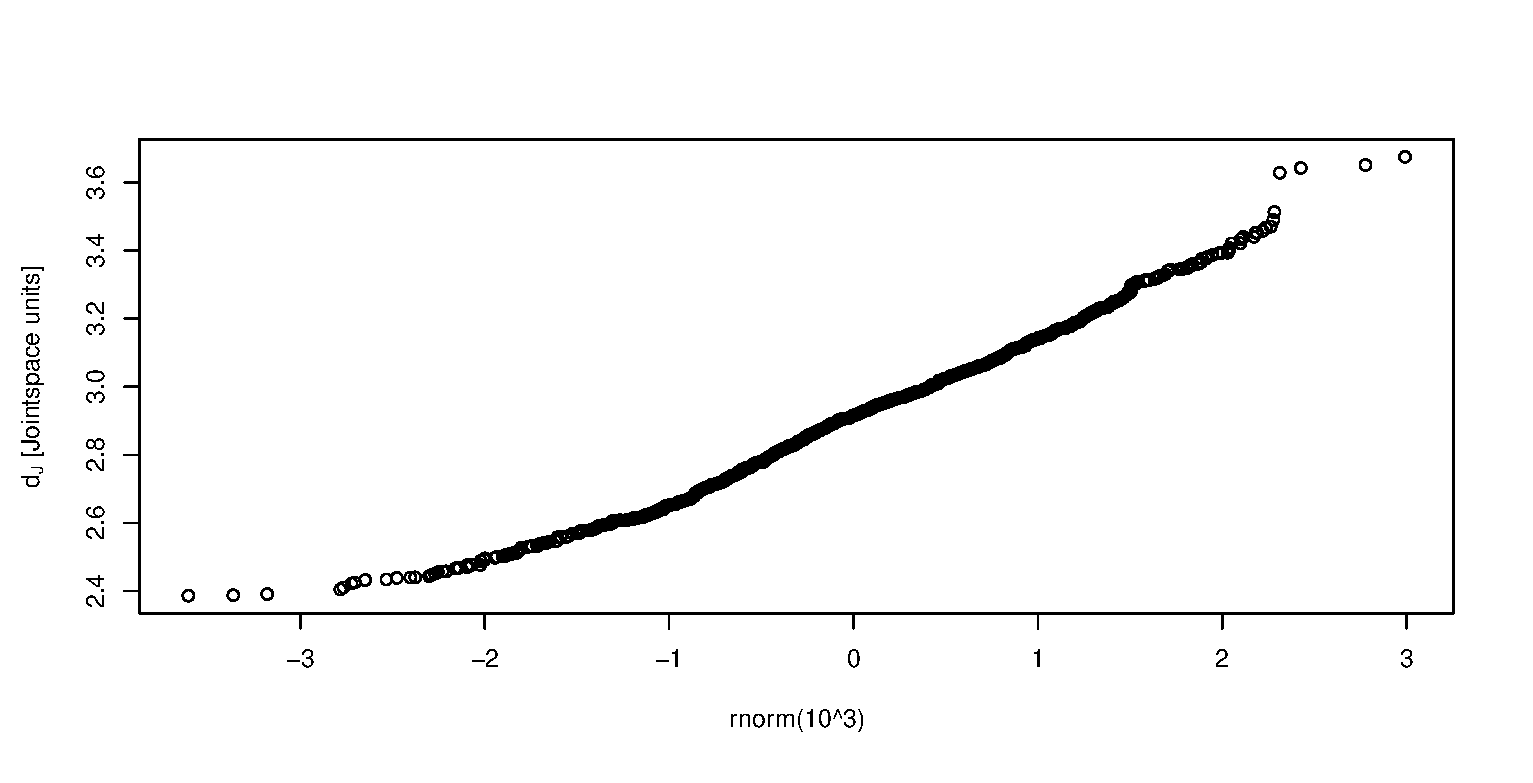
\includegraphics[width=\figsize]{graphics/qq_tran_op_ba}
 \caption{Normal QQ plot for the log transformed \(d_J\) with the optimal \(\epsilon\) for the balanced bidirectional RRT planner. The normal distribution is approximated with 1000 samples.}
 \label{fig:balanced_log_qq}
\end{figure}



